\documentclass[submit]{harvardml}
\usepackage{common}
\usepackage{float}
\course{CS1810-S26}
\assignment{Homework \#2}
\duedate{February 27, 2026 at 11:59 PM}

\usepackage[OT1]{fontenc}
\usepackage[colorlinks,citecolor=blue,urlcolor=blue]{hyperref}
\usepackage{graphicx}
\usepackage{subcaption}
\usepackage{fullpage}
\usepackage{amsmath}
\usepackage{todonotes}
\usepackage{amssymb}
\usepackage{framed}
\usepackage{color}
\usepackage{soul}
\usepackage{todonotes}
\usepackage{listings}
\usepackage{enumitem}
\usepackage{bm}
\usepackage{bbm}


\newcommand{\B}{\text{B}}
\newcommand{\Beta}{\text{Beta}}

\usepackage[mmddyyyy,hhmmss]{datetime}

\definecolor{verbgray}{gray}{0.9}

\lstnewenvironment{csv}{%
  \lstset{backgroundcolor=\color{verbgray},
  frame=single,
  framerule=0pt,
  basicstyle=\ttfamily,
  columns=fullflexible}}{}
  

%%%%%%%%%%%%%%%%%%%%%%%%%%%%%%%%%%%%%%%%%%%
%% Solution environment
\usepackage{xcolor}
\newenvironment{solution}{
    \vspace{2mm}
    \color{blue}\noindent\textbf{Solution}:
}{}
%%%%%%%%%%%%%%%%%%%%%%%%%%%%%%%%%%%%%%%%%%%


\begin{document}

\begin{center}
  {\Large Classification and Bias-Variance Trade-offs}\\
\end{center}

\subsection*{Introduction}

This homework is about classification, bias-variance trade-offs, and
uncertainty quantification.

The datasets that we will be working with relate to astronomical observations and loan applicants
The first dataset, found at \verb|data/planet-obs.csv|,
contains information on whether a planet was observed (as a binary
variable) at given points in time. This will be used in Problem 1. The
second dataset, available at \verb|data/hr.csv|, details different
loan applicants and their measured debt to income ratio and credit score. You will
work with this data in Problem 3.

As a general note, for classification problems we imagine that we have
the input matrix $\boldX \in \reals^{N \times D}$ (or perhaps they
have been mapped to some basis $\bm{\Phi}$, without loss of
generality) with outputs now ``one-hot encoded."  This means that if
there are~$K$ output classes, rather than representing the output
label $y$ as an integer~${1,2,\ldots,K}$, we represent $\boldy$ as a
``one-hot" vector of length~$K$. A ``one-hot" vector is defined as
having every component equal to 0 except for a single component which
has value equal to 1.  For example, if there are $K = 7$ classes and a
particular data point belongs to class 3, then the target vector for
this data point would be~$\boldy = [0,0,1,0,0,0,0]$.  We will define
$C_1$ to be the one-hot vector for the 1st class, $C_2$ for the 2nd
class, etc.  Thus, in the previous example $\boldy = C_3$. If there
are $K$ total classes, then the set of possible labels is $\{C_1
  \ldots C_K \} = \{C_k\}_{k=1}^K$.  Throughout the assignment we will
assume that each label $\boldy \in \{C_k\}_{k=1}^K$ unless otherwise
specified. The most common exception is the case of binary
classification ($K = 2$), in which case labels are the typical
integers $y \in \{0, 1\}$.

\subsection*{Resources and Submission Instructions}

% We encourage you to read CS181 Textbook's Chapter 3 for more information on linear classification, gradient descent, and classification in the discriminative setting. Read Chapter 2.8 for more information on the trade-offs between bias and variance.

In problems 1 and 3, you may use \texttt{numpy} or \texttt{scipy}, but not \texttt{scipy.optimize} or \texttt{sklearn}. Example code is given in the provided notebook. In past years, students have reported numerical stability issues for problem 3 and sometimes problem 1; we encourage students to not worry too much about this, as we are mindful of this in grading, but we recommend trying to run your code on \textbf{Google Colab} if you encounter issues (since this has resolved the issue for many students in the past).

Please type your solutions after the corresponding problems using this \LaTeX\ template, and start each problem on a new page. Please submit the writeup PDF to the Gradescope assignment `HW2'. Remember to assign pages for each question. \textbf{You must include any plots in your writeup PDF.} Please submit your \LaTeX file and code files to the Gradescope assignment `HW2 - Supplemental.' The supplemental files will only be checked in special cases, e.g. honor code issues, etc. Your files should be named in the same way as we provide them in the repository, e.g. \texttt{hw2.pdf}, etc.


\newpage
%%%%%%%%%%%%%%%%%%%%%%%%%%%%%%%%%%%%%%%%%%%%%
% Problem 1
%%%%%%%%%%%%%%%%%%%%%%%%%%%%%%%%%%%%%%%%%%%%%

\begin{problem}[Exploring Bias-Variance and Uncertainty, 30pts]
In this problem, we will explore the bias and variance of a few
different model classes when it comes to logistic regression, use cross validation for model selection, and
investigate two sources of predictive uncertainty in a synthetic
(made-up) scenario.

We are using a powerful telescope in the northern hemisphere to gather
measurements of some planet of interest. At certain times however, our
telescope is unable to detect the planet due to its positioning around
its star.  The data in \verb|data/planet-obs.csv| records the
observation time in the ``Time" column and whether the planet was
detected in the ``Observed" column (with the value 1 representing that
it was observed).  These observations were taken over a dark, clear
week, which is representative of the region.  Since telescope time is
expensive, we would like to build a model to help us schedule and find
times when we are likely to detect the planet.

\begin{enumerate}
\item Before we begin fitting any models, let us first derive the mathematical explanation for the bias-variance tradeoff. Let $\mathcal{D}$ denote the training dataset, while $\mathbf{x}$ is a fixed input (not in $\mathcal{D}$). Suppose the labels are generated via $$y = f(\mathbf{x}) + \varepsilon$$ where $f(\mathbf{x})$ is the true regression function and $\varepsilon$ is a noise term with $\mathbb{E}[\varepsilon|\mathbf{x}] = 0$ and $\text{Var}(\varepsilon|\mathbf{x}) = \sigma^2$. We'll denote the predictor learned from $\mathcal{D}$ as $\hat f_\mathcal{D}(\mathbf{x})$. Then, we have the prediction error as $$\text{MSE} = \mathbb{E}_{\mathcal{D}, y|\mathbf{x}}[(y - \hat f_\mathcal{D}(\mathbf{x}))^2]$$ We will see that this error decomposes into a noise term, a bias term, and a variance term. \begin{enumerate}
    \item Show that the expression for MSE above decomposes into $$\mathbb{E}_{y|\mathbf{x}}[(y - f(\mathbf{x}))^2] + \mathbb{E}_\mathcal{D}[(f(\mathbf{x}) - \hat f_\mathcal{D}(\mathbf{x}))^2] + \text{\{third term\}}$$ Hint: Add and subtract $f(\mathbf{x})$.

    \item Show that the third term from our final expression in part (b) simplifies to 0. Hint: Use Adam's Law/Law of Total Expectation.

    \item Show that the first term from our final expression in part (b) represents the noise in our data, i.e. $\mathbb{E}_{y|\mathbf{x}}[(y - f(\mathbf{x}))^2] = \sigma^2$. 

    \item Define the average predictor $\bar f(\mathbf{x}) = \mathbb{E}_\mathcal{D}[\hat f_\mathcal{D}(\mathbf{x})]$. Now show that the the second term from our final expression in part (b) represents the squared bias plus variance, i.e. $\mathbb{E}_\mathcal{D}[(f(\mathbf{x}) - \hat f_\mathcal{D}(\mathbf{x}))^2] = (f(\mathbf{x}) - \bar f(\mathbf{x}))^2 + \mathbb{E}_\mathcal{D}[(\bar f(\mathbf{x}) - \hat f_\mathcal{D}(\mathbf{x}))^2]$. 
\end{enumerate}

  \item Now let's explore the use of different bases to model our data. First, randomly split the data into 10 mini-datasets of size $N = 30$. We will use three different basis functions to model the data. We implemented basis 1 as $[1,t]$, where t is the data to help you get started. Then, choose two basis functions, which you'll use to transform the input data in the regression. (Hint: Examples of such basis functions were given in Lecture 2.) \textbf{Please write your chosen basis functions in the written section of your submission for this part of the question. }
  
  For each of these bases, fit a logistic regression model using sigmoid($\boldw^\top \boldsymbol\phi(t)$) to each dataset by using gradient descent to
        minimize the negative log-likelihood.  This means you will be
        running gradient descent 10 times for each basis, once for each
        dataset.

        Use the given starting values of $\boldw$ and a learning rate of $\eta=0.001$, take 1,000 update
        steps for each gradient descent run, and make sure to average the
        gradient over the data points at each step. These parameters,
        while not perfect, will ensure your code runs reasonably quickly.
  
  \item After consulting with a domain expert, we find that the probability of observing the planet is periodic as the planet revolves around its star---we are more likely to observe the planet when it is in front of its star than when it is behind it. In fact, the expert determines that observation follows the generating process $y \sim \text{Bern}(f(t))$, where $f(t) = 0.4 \times \cos(1.1t + 1) + 0.5$ for $t \in [0, 6]$ and $y \in \{0,1\}$. Note that we, the modelers, do not usually see the true data distribution. Knowledge of the true $f(t)$ is only exposed in this problem to allow for verification of the true bias.

        Use the given code to plot the true process versus your learned models. Include your plots in your solution PDF.

        \textbf{In no more than 5 sentences}, explain how bias and variance are reflected in the 3 types of curves on the graphs.  How do the fits of the individual and mean prediction functions change?  Keeping in mind that none of the model classes match the true generating process exactly, discuss the extent to which each of the bases approximates the true process.


    \item If we were to increase the size of each dataset drawn from $N = 30$ to a larger number, how would the bias and variance change for each basis? Why might this be the case? You may experiment with generating your own data that follows the true process and plotting the results, but this is \textbf{not} necessary. \textbf{Your response should not be longer than 5 sentences}.

    \item Consider the test point $t = 0.1$. Using your models trained on basis $\boldsymbol\phi_3$, report the predicted probability of observation of the \textit{first} model (the model trained on the first 30 data points). How can we interpret this probability as a measure of uncertainty? Then, compute the variance of the classification probability over your 10 models at the same point $t = 0.1$. How does this measurement capture another source of uncertainty, and how does this differ from the uncertainty represented by the classification probability? Repeat this process (reporting the first model's classification probability and the variance over the 10 models) for the point $t = 3.2$.

          Compare the uncertainties and their sources at times $t=0.1$ and $t=3.2$.

    \item We now need to make some decisions about when to request time on
          the telescope.  The justifications of your decisions will be sent to
          your funding agency, which will determine whether you will be
          allocated funds to use the telescope for your project. You seek out a team that has used the alternative telescope
                  for observing this planet, and they provide you their observation
                  file \verb|data/planet-obs-alternate.csv|.
                  Compare the observations from your telescope to theirs.  What
                  seems to be happening?  What might be an appropriate model for
                  this? Your funding agency asks you to refit your models on these
                  new data.  Do you think this is a reasonable ask, and if so, how
                  will it help you make better decisions about when to request
                  viewing time?  If not, why do you think the additional modeling
                  will not help? You do \emph{not} need to do any modeling; answer this question in \textbf{no more than 10 lines}. We are looking for your reasoning; there may be
          more than one valid answer.

  
      \item In part 1, we have selected 3 possible bases to use as features when training a model. This gave us 3 possible models. In this part, we will choose the right learning algorithm by using cross validation. Take your dataset split and train 10 models for each basis, using 9 of the chunks for training and 1 of the chunks for validation. Compare the average error across the 10 folds for the 3 bases. Which basis performs the best? Why do you think it performs the best?    

      
  \end{enumerate}
\end{problem}

\newpage

\begin{solution}
	\begin{enumerate}
	    \item 
        \begin{enumerate}
            \item Following the hint we show that MSE expression decomposes into the stated expression by adding and subtracting $f(x)$.
            \[
            \text{MSE} = \mathbb{E}_{\mathcal{D}, y|\mathbf{x}}[(y - \hat f_\mathcal{D}(\mathbf{x}))^2] = \mathbb{E}_{\mathcal{D}, y|\mathbf{x}}[((y-f(x)) +(f(x) - \hat f_\mathcal{D}(x)))^2]
            \]
            Let $A =(y-f(x)) $ ,and $B =(f(x) - \hat f_\mathcal{D}(x)) $. Next we expand the terms:
            \[
            MSE = \mathbb{E}_{\mathcal{D}, y|\mathbf{x}}[(y-f(x))^2] + \mathbb{E}_{\mathcal{D}, y|\mathbf{x}}[(f(x) - \hat f_\mathcal{D}(x))^2] + 2 \mathbb{E}_{\mathcal{D}, y|\mathbf{x}}[(y-f(x))(f(x) - \hat f_\mathcal{D}(x))] 
            \]

            Since the first term does not depend on the training set, and since $f(x)$ is constant in respect to $y$, then the second term does not depend on $y$ the expressions reduces to:

            \[
            MSE = \mathbb{E}_{y|\mathbf{x}}[(y-f(x))^2] + \mathbb{E}_{\mathcal{D}}[(f(x) - \hat f_\mathcal{D}(x))^2] + 2 \mathbb{E}_{\mathcal{D}, y|\mathbf{x}}[(y-f(x))(f(x) - \hat f_\mathcal{D}(x))] 
            \]

            With $2 \mathbb{E}_{\mathcal{D}, y|\mathbf{x}}[(y-f(x))(f(x) - \hat f_\mathcal{D}(x))] = \text{third term}$.
            \item From Adam's law it follows that:

            \[
            2 \mathbb{E}_{\mathcal{D}, y|\mathbf{x}}[(y-f(x))(f(x) - \hat f_\mathcal{D}(x))] =2 \mathbb{E}_{ _\mathcal{D}}[\mathbb{E}_{y|\mathbf{x}}[(y-f(x))(f(x) - \hat f_\mathcal{D}(x))]]
            \]
            Since the factor ($f(x) - \hat{f}_\mathcal{D}(x))$ does not depend on $y$
            we can write our expression as:

            \[
            2 \mathbb{E}_{\mathcal{D}, y|\mathbf{x}}[(y-f(x))(f(x) - \hat f_\mathcal{D}(x))] =2 \mathbb{E}_{ _\mathcal{D}}[(f(x) - \hat f_\mathcal{D}(x))\mathbb{E}_{y|\mathbf{x}}[(y-f(x))]]
            \]
            \medskip
            
            Since $y = f(x) +\epsilon$ then $\epsilon  =  y- f(x)$ it follows that:
            \[
                    2 \mathbb{E}_{ _\mathcal{D}}[(f(x) - \hat f_\mathcal{D}(x))\mathbb{E}_{y|\mathbf{x}}[(y-f(x))]] = 2\mathbb{E}_{\mathcal{D}}[(f(x)-\hat{f}_\mathcal{D}(x)\mathbb{E}_{\epsilon|x}(\epsilon)]
            \]

            We also now that $\mathbb{E}_{\epsilon|x} =0$. Hence,
            \[
            2 \mathbb{E}_{ _\mathcal{D}}[(f(x) - \hat f_\mathcal{D}(x))\mathbb{E}_{y|\mathbf{x}}[(y-f(x))]] = 2\mathbb{E}_{\mathcal{D}}[(f(x)-\hat{f}_\mathcal{D}(x)\mathbb{E}_{\epsilon|x}(\epsilon)] =2\mathbb{E}_{\mathcal{D}}[(f(x)-\hat{f}_\mathcal{D}(x) \cdot 0] = 0
            \]

            \item We know that $y = f(x) +\epsilon$, substituting into the expression, we get:
            \[
            \mathbb{E}_{y|\mathbf{x}}[((f(x) +\epsilon)-f(x))^2]  =\mathbb{E}_{\epsilon|\mathbf{x}}[\epsilon^2]
            \]
            Recall: Var($\epsilon | x$) = $\mathbb{E}[\epsilon^2 |x] - (\mathbb{E}[\epsilon | x])^2$, However we know that $\mathbb{E}[\epsilon |x]=0$. Hence,
            \[
            Var(\epsilon|x)= \mathbb{E}[\epsilon^2 |x] = \sigma^2.
            \]
            \item We start by adding and subtracting $\bar f(\mathbf{x})$

            \[
            \mathbb{E}_{\mathcal{D}, y|\mathbf{x}}[(f(x) - \hat f_\mathcal{D}(x))^2] =   \mathbb{E}_{\mathcal{D}, y|\mathbf{x}}[(f(x) -\bar f(\mathbf{x})) + (\bar f(\mathbf{x}) - \hat f_\mathcal{D}(x))^2]
            \]
            \[
            =
            \big(f(x) - \bar f(x)\big)^2
            +\big(\bar f(x) - \hat f_D(x)\big)^2
            +2\big(f(x) - \bar f(x)\big)\big(\bar f(x) - \hat f_D(x)\big).
            \]
            Taking expectation over $D$:
            \[
            \mathbb{E}_D[(f(x) - \hat f_D(x))^2]
            = \big(f(x) - \bar f(x)\big)^2
            + \mathbb{E}_D\big[(\bar f(x) - \hat f_D(x))^2\big]
            +2\big(f(x) - \bar f(x)\big)
            \mathbb{E}_D[\bar f(x) - \hat f_D(x)].
            \]
            
            Since
            \[
            \mathbb{E}_D[\bar f(x) - \hat f_D(x)]
            =
            \bar f(x) - \mathbb{E}_D[\hat f_D(x)]
            =
            \bar f(x) - \bar f(x)
            =
            0,
            \]
        Hence,

        \[
        \mathbb{E}_D[(f(x) - \hat f_D(x))^2]
        =
        (f(x) - \bar f(x))^2
        +
        \mathbb{E}_D[(\bar f(x) - \hat f_D(x))^2].
        \]
        \end{enumerate}
        \item For my bases, I choose a simple 4-degree polynomial base, and and a finite Fourier basis with frequency 1 it projects the 1d input into a space spanned by sine and cosine waves of increasing frequency.
        \item Observing the 10 samples fit in basis 1 we can notice that they are roughly linear and and the mean the fit of the man learned model is also roughly linear indicating high bias. Additionally, both the individual fits and the mean fit are deviating heavily from the ground truth model fit indicating low variance. However in basis 2 we can really start noticing the bias-variance tradeoff we can observe the fits are much close to the the ground truth model and has lower bias and higher variance than basis 1, however a polynomial cannot from cannot capture the periodic structure of the true generating process. Lastly for Basis 3 the individual fits differ substantially in their oscillatory behavior, indicating high variance across datasets. While the Fourier basis has the capacity to represent periodic structure and therefore low bias potential, the small sample size leads to overfitting and high variance.
        
        
        \begin{figure}[H]
        
\includegraphics[width=0.5\textwidth]{basis1.png}
        
\includegraphics[width=0.5\textwidth]{basis2.png}
        
\includegraphics[width=0.5\textwidth]{basis3.png}
        
        \end{figure}

        \item Basis 1 will remain biased however variance will decrease. Since our function is monotonic no matter how much we increase the size of our data set the best possible scenario for this model will still be "wrong". As for basis 2, variance will also drop and would approximate the sine better, still imperfectly since it's a polynomial. As for Basis 3 variance will drop significantly and this will probably become the best model, by increasing the size of our data set the model stops reacting to noise and begins to react to probability distributions.
        \item Classification probabilities for  $t = 0.1: 0.49858229125742837, t = 3.2: 0.4887376187601766$
        Model variances for $ t = 0.1: 0.00036293344824282504, t = 3.2: 0.000520494151696098$
        For t = 0.1, the first model prediction is very close to 0.5, so the model is  uncertain about the class label at that point (either outcome is about equally likely). The variance measures a different uncertainty source, the model/data uncertainty or we can think about it as how sensitive the prediction is to which 30-point dataset we happened to train on. Comparing the two points, both have similarly high classification uncertainty (because both probabilities are near 0.5) But at $t=3.2$ the variance is higher indicating higher sensitivity to the data as we progress in time.
        \item Comparing the observations recorded by the telescopes, the alternative telescope shows a higher detection rate, and a lot of consistent disagreements between the two telescope at individual timestamps(the alternative consistently reports more 1s) suggesting a telescope. A reasonable model for this would be logistic regression where each telescope his its own confusion matrix. Refitting only makes if we incorporate that telescope-specific bias (or at least we treat the alternate data as another noisy measurement) then combining both sources should reduce variance.
        \item basis1 average error (10-fold): $0.486667$ , basis2 average error (10-fold): $0.296667$, basis3 average error (10-fold): $0.516667$
        Basis2 achieves the lowest cross-validation error because it balances bias and variance. It is flexible enough to approximate the underlying sinusoidal structure better than the linear basis, while being more stable than the high-variance Fourier basis under limited data.
	\end{enumerate}
\end{solution}


\newpage
%%%%%%%%%%%%%%%%%%%%%%%%%%%%%%%%%%%%%%%%%%%%%
% Problem 2
%%%%%%%%%%%%%%%%%%%%%%%%%%%%%%%%%%%%%%%%%%%%%

\begin{problem}[Maximum likelihood in classification, 15pts]

Consider now a generative $K$-class model.  We adopt class prior
$p(\boldy = C_k; \bpi) = \pi_k$ for all $k \in \{1, \ldots, K\}$
(where $\pi_k$ is a parameter of the prior).
Let  $p(\boldx|\boldy=C_k)$ denote
the class-conditional density of features $\boldx$ (in this
case for class $C_k$). Consider the data set $\mathcal{D} = \{(\boldx_i, \boldy_i)\}_{i=1}^n$ where as above $\boldy_i \in \{C_k\}_{k=1}^K$ is
encoded as a one-hot target vector and the data are independent.

\begin{enumerate}
  \item Write out the log-likelihood of the data set, $\ln p(\mathcal{D} ; \bpi)$.

  \item Since the prior forms a distribution, it has the constraint that
        $\sum_k\pi_k - 1 = 0$.  Using the hint on
        Lagrange multipliers below, give the
        expression for the maximum-likelihood estimator for the prior
        class-membership probabilities, i.e.
        $\hat \pi_k.$
        Make sure to write out the intermediary equation you need
        to solve to obtain this estimator. Briefly state why your final answer is intuitive.
\end{enumerate}

For the remaining questions, let the
class-conditional probabilities be Gaussian distributions with
the same covariance matrix
$$p(\boldx | \boldy = C_k) = \mathcal{N}(\boldx |  \bmu_k, \bSigma), \text{\ for\ }k \in \{1,\ldots, K\}$$
and different means $\bmu_k$ for each class.

\begin{enumerate}
  \item[3.] Derive the gradient of the log-likelihood with respect to vector $\bmu_k$.
    Write the expression in matrix form as a function of the variables defined
    throughout this exercise. Simplify as much as possible for full credit.
  \item[4.] Derive the maximum-likelihood estimator $\hat{\mu}_k$ for vector $\bmu_k$. Briefly state why your final answer is intuitive.
  \item[5.] Derive the gradient for the log-likelihood with respect to the
    covariance matrix $\bSigma$ (i.e., looking
    to find an MLE for the covariance).
    Since you are differentiating with respect to a
    \emph{matrix}, the resulting expression should be a matrix!
    %
  \item[6.] Derive the maximum likelihood estimator $\hat{\Sigma}$ of the covariance matrix.
\end{enumerate}

\paragraph{Hint: Lagrange Multipliers.} Lagrange Multipliers are a method for
optimizing a function $f$ with respect to an
equality constraint, i.e.
\[\min_{\boldx} f(\boldx)\ \text{s.t.}\ g(\boldx) = 0.\]

This can be turned into an unconstrained problem by introducing a
Lagrange multiplier $\lambda$ and constructing the Lagrangian function,
\[L(\boldx, \lambda) =  f(\boldx) + \lambda g(\boldx).\]

It can be shown that it is a necessary condition that the optimum
is a critical point of this new function. We can find this point by solving two equations:

\[\frac{\partial L(\boldx, \lambda)}{\partial  \boldx} = 0  \ \ \text{and}\  \  \frac{\partial L(\boldx, \lambda)}{\partial \lambda} = 0 \]


\paragraph{Cookbook formulas.} Here are some formulas you might want to consider
using to compute difficult gradients. You can use them  in the homework
without proof. If you are looking to hone your matrix calculus skills, try to
find different ways to prove these formulas yourself (will not be part of the
evaluation of this homework). In general, you can use any formula from the matrix cookbook,
as long as you cite it. We opt for the following common notation:
$\boldX^{-\top} := (\boldX^{\top})^{-1}$
\begin{align*}
   & \frac{\partial \bolda^\top \boldX^{-1} \boldb}{\partial \boldX} = - \boldX^{-\top} \bolda \boldb^\top \boldX^{-\top} \\
   & \frac{\partial \ln | \det (\boldX) |}{\partial \boldX} = \boldX^{-\top}
\end{align*}

These formulas are from the matrix cookbook linked here: \href{https://www.math.uwaterloo.ca/~hwolkowi/matrixcookbook.pdf}{The Matrix Cookbook (University of Waterloo)}.  
\end{problem}


\newpage

\begin{solution}
	\begin{enumerate}
	    \item $\ln p(D;\pi)
=
\sum_{i=1}^{n}
\sum_{k=1}^{K}
y_{ik}
\left(
\ln \pi_k
+
\ln p(x_i \mid y = C_k)
\right).$
\item \[
\ell(\pi)
=
\sum_{i=1}^{n}
\sum_{k=1}^{K}
y_{ik} \ln \pi_k
=
\sum_{k=1}^{K}
N_k \ln \pi_k,
\quad
\text{where }
N_k = \sum_{i=1}^{n} y_{ik}.
\]

\[
\text{Constraint: }
\sum_{k=1}^{K} \pi_k - 1 = 0.
\]

\[
\mathcal{L}(\pi,\lambda)
=
\sum_{k=1}^{K} N_k \ln \pi_k
+
\lambda
\left(
\sum_{k=1}^{K} \pi_k - 1
\right).
\]

\[
\frac{\partial \mathcal{L}}{\partial \pi_k}
=
\frac{N_k}{\pi_k}
+
\lambda
= 0
\quad
\Rightarrow
\quad
\pi_k
=
-\frac{N_k}{\lambda}.
\]

\[
\frac{\partial \mathcal{L}}{\partial \lambda}
=
\sum_{k=1}^{K} \pi_k - 1
= 0.
\]

Substituting:

\[
\sum_{k=1}^{K}
\left(
-\frac{N_k}{\lambda}
\right)
=
1
\quad
\Rightarrow
\quad
-\frac{1}{\lambda}
\sum_{k=1}^{K} N_k
=
1.
\]

Since
\[
\sum_{k=1}^{K} N_k = n,
\]

we obtain

\[
-\frac{n}{\lambda} = 1
\quad
\Rightarrow
\quad
\lambda = -n.
\]

Therefore,
\[
\hat{\pi}_k
=
\frac{N_k}{n}
=
\frac{1}{n}
\sum_{i=1}^{n} y_{ik}.
\]


Thus, the MLE of  $\pi_k$ is the empirical fraction of samples in class  $k$ making intuitive.
\item \[
\ell(\mu_k)
=
\sum_{i=1}^{n}
y_{ik}\log \mathcal{N}(x_i \mid \mu_k,\Sigma).
\]

Using the Gaussian log-density,

\[
\log \mathcal{N}(x_i \mid \mu_k,\Sigma)
=
-\frac{1}{2}
(x_i-\mu_k)^\top \Sigma^{-1} (x_i-\mu_k)
+ \text{const},
\]

we obtain

\[
\ell(\mu_k)
=
-\frac{1}{2}
\sum_{i=1}^{n}
y_{ik}
(x_i-\mu_k)^\top \Sigma^{-1} (x_i-\mu_k)
+ \text{const}.
\]

Using the identity
\[
\frac{\partial}{\partial \mu}
\big[(x-\mu)^\top A (x-\mu)\big]
=
-2A(x-\mu)
\quad (\text{for symmetric }A),
\]

with \(A=\Sigma^{-1}\), the gradient is

\[
\nabla_{\mu_k} \ell
=
\sum_{i=1}^{n}
y_{ik}\Sigma^{-1}(x_i-\mu_k).
\]

Factoring out \(\Sigma^{-1}\),

\[
\nabla_{\mu_k} \ell
=
\Sigma^{-1}
\left(
\sum_{i=1}^{n} y_{ik} x_i
-
\mu_k \sum_{i=1}^{n} y_{ik}
\right).
\]

Let
\[
N_k = \sum_{i=1}^{n} y_{ik}.
\]

Then the gradient simplifies to

\[
\nabla_{\mu_k} \ell
=
\Sigma^{-1}
\left(
\sum_{i=1}^{n} y_{ik} x_i
-
N_k \mu_k
\right).
\]

In matrix form, letting \(X \in \mathbb{R}^{n\times d}\) contain rows \(x_i^\top\) and
\(y_k \in \mathbb{R}^n\) be the vector with entries \(y_{ik}\),

\[
\nabla_{\mu_k} \ell
=
\Sigma^{-1}
\left(
X^\top y_k
-
N_k \mu_k
\right).
\]
\item \[
\ell(\mu_k)
=
\sum_{i=1}^{n}
y_{ik}\log \mathcal{N}(x_i \mid \mu_k,\Sigma)
=
-\frac{1}{2}
\sum_{i=1}^{n}
y_{ik}(x_i-\mu_k)^\top \Sigma^{-1}(x_i-\mu_k)
+\text{const}.
\]

From the previous result,
\[
\nabla_{\mu_k}\ell
=
\sum_{i=1}^{n} y_{ik}\Sigma^{-1}(x_i-\mu_k)
=
\Sigma^{-1}\left(\sum_{i=1}^{n} y_{ik}x_i - \mu_k\sum_{i=1}^{n} y_{ik}\right).
\]

Set the gradient to zero:
\[
\Sigma^{-1}\left(\sum_{i=1}^{n} y_{ik}x_i - \mu_k\sum_{i=1}^{n} y_{ik}\right)=0
\quad\Longrightarrow\quad
\sum_{i=1}^{n} y_{ik}x_i - \mu_k\sum_{i=1}^{n} y_{ik}=0.
\]

Let \(N_k=\sum_{i=1}^{n} y_{ik}\). Solving for \(\mu_k\) gives the MLE:
\[
\hat{\mu}_k
=
\frac{1}{N_k}\sum_{i=1}^{n} y_{ik}x_i.
\]

\item \[
\ell(\Sigma)
=
\sum_{i=1}^{n}
\sum_{k=1}^{K}
y_{ik}
\log \mathcal{N}(x_i \mid \mu_k,\Sigma).
\]

Using the Gaussian log-density,

\[
\log \mathcal{N}(x_i \mid \mu_k,\Sigma)
=
-\frac{1}{2}
\log |\Sigma|
-\frac{1}{2}
(x_i-\mu_k)^\top \Sigma^{-1}(x_i-\mu_k)
+ \text{const},
\]

we obtain

\[
\ell(\Sigma)
=
-\frac{1}{2}
\sum_{i=1}^{n}
\sum_{k=1}^{K}
y_{ik}
\left[
\log |\Sigma|
+
(x_i-\mu_k)^\top \Sigma^{-1}(x_i-\mu_k)
\right]
+ \text{const}.
\]

Let \(N = \sum_{i=1}^{n}\sum_{k=1}^{K} y_{ik} = n\).
Using the matrix identities

\[
\frac{\partial}{\partial \Sigma}\log|\Sigma|
=
\Sigma^{-T},
\qquad
\frac{\partial}{\partial \Sigma}
\left[
(x-\mu)^\top \Sigma^{-1}(x-\mu)
\right]
=
-\Sigma^{-T}(x-\mu)(x-\mu)^\top\Sigma^{-T},
\]

we obtain

\[
\nabla_{\Sigma}\ell
=
-\frac{1}{2}
\left[
\sum_{i=1}^{n}\sum_{k=1}^{K}
y_{ik}\Sigma^{-T}
-
\sum_{i=1}^{n}\sum_{k=1}^{K}
y_{ik}
\Sigma^{-T}(x_i-\mu_k)(x_i-\mu_k)^\top\Sigma^{-T}
\right].
\]

Factoring out \(\Sigma^{-T}\),

\[
\nabla_{\Sigma}\ell
=
-\frac{1}{2}
\Sigma^{-T}
\left[
N I
-
\sum_{i=1}^{n}\sum_{k=1}^{K}
y_{ik}(x_i-\mu_k)(x_i-\mu_k)^\top
\Sigma^{-T}
\right].
\]

A cleaner equivalent expression is

\[
\nabla_{\Sigma}\ell
=
\frac{1}{2}
\Sigma^{-T}
\left[
\sum_{i=1}^{n}\sum_{k=1}^{K}
y_{ik}(x_i-\mu_k)(x_i-\mu_k)^\top
-
N\Sigma
\right]
\Sigma^{-T}.
\]

\item \[
\ell(\Sigma)
=
-\frac{1}{2}
\sum_{i=1}^{n}\sum_{k=1}^{K}
y_{ik}
\left[
\log|\Sigma|
+
(x_i-\mu_k)^\top \Sigma^{-1}(x_i-\mu_k)
\right]
+\text{const}.
\]

From the previous question, the gradient can be written as
\[
\nabla_{\Sigma}\ell
=
\frac{1}{2}\Sigma^{-T}
\left[
\sum_{i=1}^{n}\sum_{k=1}^{K}
y_{ik}(x_i-\mu_k)(x_i-\mu_k)^\top
-
n\Sigma
\right]
\Sigma^{-T}.
\]

Setting the gradient to zero and using that \(\Sigma^{-T}\) is invertible,
\[
\sum_{i=1}^{n}\sum_{k=1}^{K}
y_{ik}(x_i-\mu_k)(x_i-\mu_k)^\top
-
n\Sigma
=
0.
\]

Solving for \(\Sigma\) gives the maximum-likelihood estimator
\[
\hat{\Sigma}
=
\frac{1}{n}
\sum_{i=1}^{n}\sum_{k=1}^{K}
y_{ik}(x_i-\mu_k)(x_i-\mu_k)^\top.
\]

Equivalently, letting \(N_k=\sum_{i=1}^{n}y_{ik}\),
\[
\hat{\Sigma}
=
\frac{1}{n}
\sum_{k=1}^{K}
\sum_{i:\,y_i=C_k}
(x_i-\hat{\mu}_k)(x_i-\hat{\mu}_k)^\top.
\] 

	\end{enumerate}
\end{solution}

\newpage
%%%%%%%%%%%%%%%%%%%%%%%%%%%%%%%%%%%%%%%%%%%%%
% Problem 3
%%%%%%%%%%%%%%%%%%%%%%%%%%%%%%%%%%%%%%%%%%%%%

\begin{problem}[Classifying Loan Applicants, 30pts]
In this problem, you will code up three different classifiers to classify different types of loan applicants. The file \verb|data/hr.csv| contains data on debt to income ratio measured in tenths of a percent and credit score. The data can be plotted on these two axes:
\begin{center}
  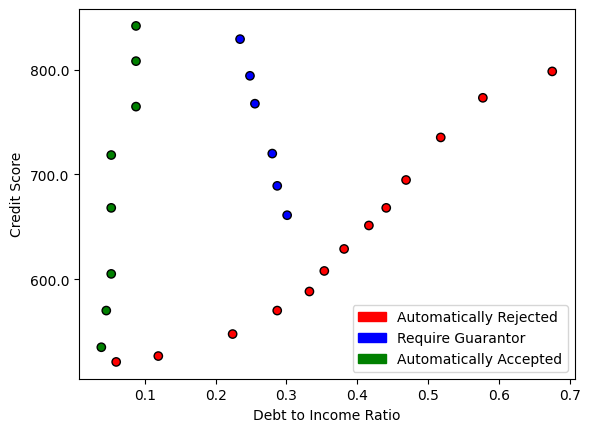
\includegraphics[width=.5\textwidth]{img_input/credit.png}
\end{center}
We've further transformed the raw data on debt to income ratio and credit score so that the default feature vector that you will be working with is defined as such:
\[\bm{x} = \left[\text{debt\_income\_ratio} \cdot \frac{200}{7}-7.5, \frac{\text{credit\_score}-500}{140}+0.5\right]^\top\]

\noindent Please implement the following classifiers:


\begin{enumerate}[label=\alph*)]

  \item \textbf{A generative classifier with Gaussian class-conditional
          densities with a \textit{shared covariance} matrix} across all classes.
        Feel free to re-use your Problem 2 results.

  \item \textbf{Another generative classifier with Gaussian class-conditional densities , but now
          with a \textit{separate covariance} matrix} learned for each class. (Note:
        The staff implementation can switch between the two Gaussian generative classifiers with just a
        few lines of code.)

  \item \textbf{A multi-class logistic regression classifier} using the softmax activation function. In your implementation of gradient descent, \textbf{make sure to use L2 regularization} with regularization parameter $\lambda = 0.001$. Please also include a \emph{\textbf{bias term, but do not regularize it}}. Limit the number of iterations of gradient descent to 200,000, and set the learning rate to be $\eta = 0.001$.

  \item \textbf{Another multi-class logistic regression classifier} with the additional feature map:
  $$\phi(\bm x) = [\ln (x_1+10), x_2^2]^\top$$

  \item \textbf{A kNN classifier} in which you classify based on the $k = 1$ and $k = 5$ nearest neighbors and the following distance function: 
  \[\text{dist}(\boldsymbol{x}, \boldsymbol{x}') = (x_1 - x'_1)^2/9 + (x_2 - x'_2)^2\]
        where nearest neighbors are those with the smallest distances from a given point.

        Note 1: When there are more than two labels, no label may have the
        majority of neighbors.  Use the label that has the most votes among
        the neighbors as the choice of label.

        Note 2: The grid of points for which you are making predictions
        should be interpreted as our test space.  Thus, it is not necessary
        to make a test point that happens to be on top of a training point
        ignore itself when selecting neighbors.

\end{enumerate}

After implementing the above classifiers, complete the following exercises:
  \begin{enumerate}



      \item Plot the decision boundaries generated by each classifier for the dataset. Include them in your PDF.
            Identify the similarities and differences among the classifiers. What explains the differences---in particular, which aspects or properties of each model dictate the shape of its decision boundary?
    
      \item
    
            Consider a loan applicant with Debt to Income Ratio 0.32 and Credit Score 350. To which class does each classifier assign this applicant? Report the classification probabilities of this applicant for models (c) and (d).
            
            Interpret how each model makes its classification decision. What else should we, the modelers, be aware of when making predictions on a point “far” from our training data? \textbf{Your response should no be longer than 5 sentences.}

    \item
        Can you think of any ethical problem that might arise from using this classifier to make loan decisions? You may approach this from any angle you like. For instance, can you think of someone who might have a low credit score and high debt-to-income ratio that you believe should nonetheless be offered a loan? Are there other variables that should be accounted for to ensure fair decisions? Are credit scores and debt-to-income ratio good bases for loan decisions? More generally, is using a classifier trained on past decisions to determine loan eligibility problematic in any way?
    \end{enumerate}
\end{problem}

\newpage

\begin{solution}
	\begin{enumerate}
	    \item The Gaussian model with shared covariance and the raw softmax classifier both produce linear decision boundaries because they are linear functions of the input features. The Gaussian model with separate covariances produces curved boundaries due to class-specific quadratic terms. The softmax classifier with the nonlinear feature map produces nonlinear boundaries because it is linear in the transformed feature space but nonlinear in the original space. kNN produces highly irregular boundaries, especially for $k=1$, because it is non-parametric and makes decisions based purely on local neighborhoods. Increasing $k$ smooths the boundary by reducing variance through local averaging. \begin{figure}[H]
	    \centering
	    
\includegraphics[width=0.3\linewidth]{softmax_phi.png} 
\includegraphics[width=0.3\linewidth]{softmax_raw.png}
        
\includegraphics[width=0.3\linewidth]{knn_k1.png}
        
\includegraphics[width=0.3\linewidth]{knn_k5.png}
        
\includegraphics[width=0.3\linewidth]{gaussian_separate.png}
        
\includegraphics[width=0.3\linewidth]{gaussian_shared.png}
	\end{figure}
    \item Model (c) prediction: $[0]$
Model (c) probabilities: $[[9.99999653e-01 3.47070714e-07 2.82260310e-10]]$
Model (d) prediction: $[1]$
Model (d) probabilities: $[[0.2538532  0.65886064 0.08728616]]$. The difference arises because model (c) is linear in the original feature space, while model (d) is linear in a transformed nonlinear feature space, leading to different decision geometry.
\item Using a classifier trained on past loan decisions risks perpetuating historical biases, especially if past approvals reflected systemic discrimination (historical racial/gender based discrimination and whatnot). Credit scores and debt-to-income ratios are correlated with socioeconomic and demographic factors, potentially leading to discrimination and unintended biases. 
		\end{enumerate}
\end{solution}

\newpage

\begin{problem}[Gradient Descent and Regularization, 15pts]

\noindent In this problem, you will analyze gradient descent for linear regression and study how \emph{ridge regularization} modifies the optimization landscape. You will first derive gradient descent updates for ordinary least squares, then extend them to the ridge-regularized objective. Finally, you will implement these algorithms to empirically observe how regularization affects convergence and generalization.

\medskip

\noindent Consider a regression dataset $\mathcal D = \{(\mathbf x_i, y_i)\}_{i=1}^N$, where each input $\mathbf x_i \in \mathbb{R}^D$ and response $y_i \in \mathbb{R}$. Let $\mathbf X \in \mathbb{R}^{N \times D}$ denote the design matrix and let $\mathbf y \in \mathbb{R}^N$ denote the vector of responses.
\\\\
\textbf{Detail:} The predictors in this dataset are \emph{highly correlated}.
As a result, the ordinary least squares objective may be ill-conditioned,
which can lead to unstable gradient descent updates and high-variance
parameter estimates. In later parts of this problem, we will examine how
ridge regularization modifies the optimization landscape in this setting.
\\\\
\noindent Consider the ordinary least squares objective
\begin{equation*}
    \mathcal L(\mathbf w) = \frac{1}{2} \|\mathbf X\mathbf w - \mathbf y\|_2^2.    
\end{equation*}

\begin{enumerate}

\item Derive the gradient $\nabla_{\mathbf w} \mathcal L(\mathbf w)$ with respect to the parameter vector $\mathbf w$. Your final expression should be written in matrix/vector form and simplified as much as possible.

\item Using your result, write the full-batch gradient descent update rule for
$\mathbf w$ with step size $\eta > 0$.
\\\\
\noindent Now consider the ridge-regularized objective
\begin{equation*}
    \mathcal L_\text{ridge}(\mathbf w) = \frac{1}{2} \|\mathbf X\mathbf w - \mathbf y\|_2^2 + \frac{\lambda}{2} \|\mathbf w\|_2^2,
\end{equation*}
where $\lambda \ge 0$ is a regularization parameter. Important note: typically, we do not regularize the bias term, $w_0$, thus $\|\mathbf w\|_2^2$ should be replace with $\mathbf w'$ where $w'_0 = 0$. However, for the sake of simplicity, we will omit that detail for the rest of the problem.

\item Derive the gradient $\nabla_{\mathbf w}\mathcal L_\text{ridge}(\mathbf w)$. Clearly indicate how the regularization term modifies the gradient compared to the unregularized case.


\item Rewrite the update in a form that makes the effect of ridge regularization
explicit. Briefly explain how this form illustrates the shrinkage effect of the
regularization term on the parameters.

\item You will implement gradient descent for both the ordinary least squares and
ridge-regularized objectives derived above and empirically study the effect of
regularization. Specifically, you will

\begin{itemize}
    \item Implement gradient and loss functions for both regular and ridge regression
    \item Write update step functions for stochastic gradient descent, stochastic gradient descent + momentum, and Adam optimizer.
\end{itemize}

Try not to touch anything that is not in between ``\textit{sol}" and ``\textit{los}"!


\item Generate the contour plots for the trajectories of the three algorithms across both the regularized and non-regularized case. What do you notice about the speed of convergence as well as where the algorithms converge to? What do you notice about the geometry of the loss function?\\
\textit{Note: the graphing code will pause when the first descent converges, so we see that some will not converge. Also, you'll see a subspace for the optimum in the unregularized case since we have a non-full rank data matrix $\mathbf X$!}

\end{enumerate}
\end{problem}

\pagebreak

\begin{solution}
	\begin{enumerate}
	    \item \[\;L(w)=\frac{1}{2}\|Xw-y\|_2^2=\frac{1}{2}(Xw-y)^\top (Xw-y)\;\]
\[\;L(w)=\frac{1}{2}\left(w^\top X^\top Xw-2y^\top Xw+y^\top y\right)\;\]
\[\;\nabla_w L(w)=\frac{1}{2}\left(2X^\top Xw-2X^\top y\right)\;\]
\[\;\nabla_w L(w)=X^\top Xw-X^\top y\;\]
\[\;\nabla_w L(w)=X^\top (Xw-y)\;\]
\item \[\;w^{(t+1)}=w^{(t)}-\eta\,\nabla_w L\!\left(w^{(t)}\right)\;\]
\[\;\nabla_w L(w)=X^\top(Xw-y)\;\]
\[\;w^{(t+1)}=w^{(t)}-\eta\,X^\top\!\left(Xw^{(t)}-y\right)\;\]

\[\;L_{\text{ridge}}(w)=\frac{1}{2}\|Xw-y\|_2^2+\frac{\lambda}{2}\|w\|_2^2\;\]
\[\;\nabla_w L_{\text{ridge}}(w)=X^\top(Xw-y)+\lambda w\;\]
\[\;w^{(t+1)}=w^{(t)}-\eta\left[X^\top\!\left(Xw^{(t)}-y\right)+\lambda w^{(t)}\right]\;\]

\item \[\;L_{\text{ridge}}(w)=\frac{1}{2}\|Xw-y\|_2^2+\frac{\lambda}{2}\|w\|_2^2\;\]
\[\;\nabla_w\left(\frac{1}{2}\|Xw-y\|_2^2\right)=X^\top(Xw-y)\;\]
\[\;\nabla_w\left(\frac{\lambda}{2}\|w\|_2^2\right)=\frac{\lambda}{2}\nabla_w(w^\top w)=\frac{\lambda}{2}(2w)=\lambda w\;\]
\[\;\nabla_w L_{\text{ridge}}(w)=X^\top(Xw-y)+\lambda w\;\]
Compared to the unregularized gradient $X^\top(Xw-y)$, ridge adds the term $+\lambda w.$
\item \[\;w^{(t+1)}=w^{(t)}-\eta\left[X^\top(Xw^{(t)}-y)+\lambda w^{(t)}\right]\;\]
\[\;w^{(t+1)}=w^{(t)}-\eta X^\top(Xw^{(t)}-y)-\eta\lambda w^{(t)}\;\]
\[\;w^{(t+1)}=(1-\eta\lambda)w^{(t)}-\eta X^\top(Xw^{(t)}-y)\;\]
Thus ridge multiplies the current weights by $(1-\eta\lambda)$before the gradient step, causing shrinkage toward zero.
\item In the unregularized case, the loss surface contains a flat hill, so the algorithms converge slowly and may end at different points along a subspace of minimizers; with ridge regularization, the loss becomes strictly convex with a unique minimum, improving conditioning and leading to faster, more stable convergence, particularly for Momentum and Adam. SGD remains slower overall.
\begin{figure}[H]
    \centering 
    
\includegraphics[width=0.8\linewidth]{output.png}
   
\end{figure}
	\end{enumerate}
\end{solution}


%%%%%%%%%%%%%%%%%%%%%%%%%%%%%%%%%%%%%%%%%%%%%
% Name and Calibration
%%%%%%%%%%%%%%%%%%%%%%%%%%%%%%%%%%%%%%%%%%%%%

\pagebreak
\textbf{Name}: Ibrahim Khaliliya 

\textbf{Collaborators and Resources}: 
(lecture slides, section 2 and 3blue1brown )
\end{document}
